\documentclass[../elettronica]{subfiles}

\begin{document}
\section{Diodo a giunzione PN}
\subsection{Diodo}
\begin{center}
    \begin{circuitikz}
        \draw (0, 0) to[diode, *-*] (2, 0);
    \end{circuitikz}
\end{center}

Il diodo è un componente la cui corrente ha una formula esponenziale, dipendente dalla tensione applicata ai suoi capi:
\[
    I = \diodecurrent{V}
\]
Dall'espressione è possibile notare come per $V \to -\infty$, la corrente tende asintoticamente al valore $-I_S$, detto \textit{corrente di saturazione}.
\\
Dato che $I_S$ assume valori molto bassi, sull'ordine di $10^{-15}$, si può trascurare rispetto
al resto delle correnti che circolano nel circuito, approssimandola a 0.

Per $V > V_T$ la corrente esponenziale inizia a prevalere rispetto alla corrente di saturazione.
È possibile quindi distinguere due regioni di funzionamento: una valida per $V < V_T$ caratterizzata da una bassa corrente, ed una caratterizzata da una corrente elevata, valida per $V > V_T$. Le due regioni prendono il nome di \textit{polarizzazione diretta} e \textit{polarizzazione inversa}.

Diremo che il diodo è spento (non fa passare corrente) in regione di polarizzazione inversa, mentre diremo che è acceso in regione di polarizzazione diretta.

\subsubsection{Analisi del circuito raddrizzatore a singola semionda}
\begin{figure}[h]
    \centering
    \begin{tikzpicture}[/tikz/circuitikz/bipoles/length=1cm, scale=1.1]
        \draw
            (0, 0) node[ground]{}
            -- (-1, 0)
            to [american voltage source, v=$V_i$, i=I] (-1, 2)
            to [diode, v^=$V_d$, i=$I_D$] (+1, 2)
            to [R, v^=$V_u$](1, 0)
            -- (0, 0)
            ;
    \end{tikzpicture}
    \caption{Raddrizzatore a singola semionda}
    \label{fig:singola_semionda}
\end{figure}

Il circuito in figura è descritto dalle relazioni:
\[
    \begin{cases}
        V_i = V_d + V_u
        \\
        I_D = \diodecurrent{V_d}
        \\
        I = I_D
    \end{cases}
\]
$V_T$ indica la tensione termica del diodo: $V_T = K \frac{T}{q}$, con $K$ costante di Boltzmann, $q$ la carica di un elettrone e
$T$ la temperatura del circuito (misurata a temperatura ambiente: $300K$).
\\
Siccome è prodotto di costanti, $V_T$ è considerabile come una costante approssimabile a $26mV$.

Svolgendo il sistema otteniamo l'equazione
\[
    V_u = R I_S (e^{\frac{V_i - V_u}{V_T}} -1)
\]
Risolvendo per $V_i$
\[
    V_i = V_u + V_T \ln(V_u + R I_S)
\]
Otteniamo che $V_i$ è composto dalla somma tra un componente lineare ed uno logaritmico, possiamo quindi tracciare un grafico approssimato di $V_i(V_u)$ e per ottenere $V_u(V_i)$ basta effettuare una simmetria sulla bisettrice:

\begin{center}
    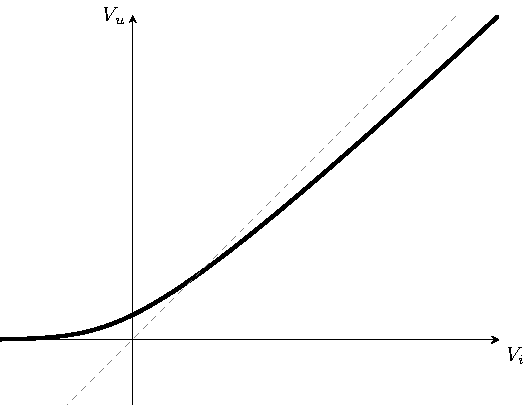
\includegraphics{diode-voltage}
\end{center}

\subsection{Modello a soglia}
Per semplificare la risoluzione dei circuiti con diodo, possiamo studiare le due regioni di funzionamento separatamente,
approssimando le due regioni di funzionamento del diodo con delle semirette.
Il primo descritto dalla caratteristica $I = 0$ (diodo spento) valido per $V_d < V_\gamma$, ed il secondo una semiretta
perpendicolare alle ascisse $V = V_\gamma$ a rappresentare la corrente costante a diodo acceso.
\warnbox{
    \begin{tabular*}{.7\textwidth}{@{\extracolsep{\fill}} cc}
        \textbf{P. INVERSA (off)} & \textbf{P. DIRETTA (on)}\\
        $\diodeoffcases{I}{V}$ & $\diodeoncases{I}{V}$\\
    \end{tabular*}
}
Questa semplificazione porta a dover risolvere il circuito due volte, una per ogni stato di funzionamento in cui
il diodo si può trovare. Inoltre è necessario anche controllare le relative ipotesi di funzionamento.

Partendo dall'ipotesi che il diodo sia spento, $\vu = R \cdot I = 0$.
Inoltre abbiamo che $V_d = \vi - \cancel{\vu} = \vi$, e per ipotesi di funzionamento $V_d < \vgg$, quindi il diodo
è spento per $\vi < \vgg$.

Studiando ora la seconda ipotesi, diodo acceso, abbiamo che:
$V_u = V_i - V_d = V_i - \vgg$. E come condizioni di validità:
\[
    \begin{cases}
        V_u = R \cdot I\\
        I \cdot R > 0\\
        V_u = V_i - V_d
    \end{cases} \quad \Rightarrow \quad V_i - V_d > 0 \quad \Rightarrow {\color{clr-main-blue}{V_i > V_d}}
\]
\subsubsection{Grafico dell'uscita ed andamento del circuito con ingresso sinusoidale}
\begin{figure}[h]
    \centering
    \begin{minipage}[b]{0.48\textwidth}
        \begin{tikzpicture}
            \begin{axis}[xlabel=$V_i$, ylabel=$V_u$, ymin=-1, width={.9\textwidth}]
                \addplot[clr-main-red, domain=-50:0.78]{0};
                \addplot[clr-main-blue, domain=0.78:50]{x - 0.78};
                \node[label={$V_\gamma$},circle,fill,inner sep=1.5pt] at (axis cs: 0.78,0) {};
            \end{axis}
        \end{tikzpicture}
    \end{minipage}%
    \begin{minipage}[b]{.48\textwidth}
        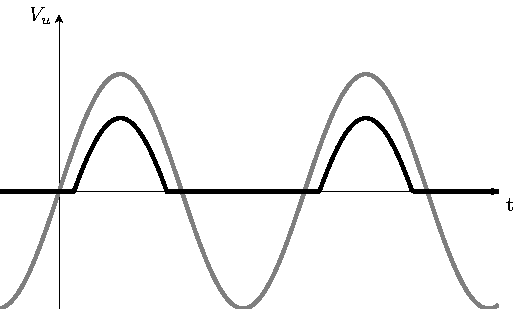
\includegraphics[width=\textwidth]{graph_raddrizzatore_singola_semionda}
    \end{minipage}
\end{figure}

\newpage
\subsection{Circuito limitatore di tensione}
\begin{figure}[h]
    \centering
    \begin{circuitikz}
        \draw (0, 0) node[circ]{}
            node[left]{$V_i$}
            -- (.2, 0)
            to[R] ++(0, -1.5)
            -- ++(.2, 0) node[circ]{} node[right]{$V_u$}
            (.2, -1.5)
            to[diode] ++(0, -1.5)
            node[ground]{};
    \end{circuitikz}
\end{figure}

\begin{minipage}[b]{.50\textwidth -1.11pt}
    \begin{tcolorbox}[title=Diodo OFF]
        \[
            I = 0 \Rightarrow
            \begin{cases}
                V_i = V_u \\
                V_u < V_\gamma
            \end{cases}
        \]
    \end{tcolorbox}
\end{minipage}
\begin{minipage}[b]{.50\textwidth -1.11pt}
    \begin{tcolorbox}[title=Diodo ON]
        \[
            \begin{cases}
                V_u = V_\gamma \\
                I_D = \frac{V_i - V_\gamma}{R} > 0
                \Rightarrow V_i > V_\gamma
            \end{cases}
        \]
    \end{tcolorbox}
\end{minipage}
Possiamo osservare che se il segnale in ingresso eccede $V_\gamma$, il diodo si accende e limita l'uscita a $V_\gamma$. Da questo il nome \textit{circuito limitatore di tensione}.

\begin{figure}[h]
    \centering
    \begin{minipage}[b]{0.48\textwidth}
        \begin{tikzpicture}
            \begin{axis}[xlabel=$V_i$, ylabel=$V_u$, ymax=2, ymin=-2.5, width={.9\textwidth}]
                \addplot[clr-main-red, domain=-5:0.78]{x};
                \addplot[clr-main-blue, domain=0.78:5]{0.78};
                \addplot[clr-gray, dashed] coordinates {(0.78, -4) (0.78, 1)};
                \node[label={-45:{$V_\gamma$}},circle,fill,inner sep=1.5pt] at (axis cs: 0.78,0) {};
            \end{axis}
        \end{tikzpicture}
    \end{minipage}%
    \begin{minipage}[b]{.48\textwidth}
        \begin{tikzpicture}[
            declare function={
                func(\x) = (\x < 0.78) * \x + (\x >= 0.78) * 0.78;
            }]
            \begin{axis}[xlabel=$V_i$, ylabel=$V_u$, ymax=2, ymin=-2.5, width={.9\textwidth}]
                \addplot[clr-main-blue, samples=30]{func(2*sin(deg(x)))};
                \addplot [clr-gray, dashed]{0.78};
            \end{axis}
        \end{tikzpicture}
    \end{minipage}
\end{figure}

% Lezione 3
\newpage
\subsection{Circuito limitatore inferiore}
\begin{figure}[h]
    \centering
    \begin{circuitikz}
        \draw (0.5, 0) node[ground]{}
            -- (-1, 0)
            to[american voltage source, label=$V_i$] (-1, 2.5)
            to[R, v>=$V_R$] (2, 2.5);
        \draw (0.5, 0)
            -- (2, 0)
            to[battery2, label=$V_b$] (2, 1)
            to[diode, i=$I$, v=$V_d$] (2, 2.5);

        \draw (3, 2.5) to[open, v^=$V_u$] (3, 0);
    \end{circuitikz}
\end{figure}

\begin{tcolorbox}[title=Diodo OFF]
    \[
        \diodeoffcases{I}{V_d}
        \cup
        \begin{cases}
            V_i = V_u - V_R
            \\
            V_u = V_b - V_d
        \end{cases}
        \Rightarrow
        \begin{cases}
            {\color{clr-main-blue}V_i = V_u}
            \\
            V_i > V_b - V_\gamma
        \end{cases}
    \]
\end{tcolorbox}
\begin{tcolorbox}[title=Diodo ON]
    \[
        \diodeoncases{I}{V_d}
        \cup
        \begin{cases}
            V_i = V_u - V_R
            \\
            V_u = V_b - V_d
        \end{cases}
        \Rightarrow
        \begin{cases}
            {\color{clr-main-red}V_u = V_b - V_\gamma}
            \\
            V_i < V_b - V_\gamma
        \end{cases}
    \]
\end{tcolorbox}
\noindent Il circuito effettua una limitazione sui valori bassi, e la soglia di intervento è regolabile dal parametro $V_b$.

\begin{figure}[h]
    \centering
    \def\vg{3 -\vgamma}
    \begin{minipage}[b]{.48\textwidth}
        \begin{tikzpicture}
            \begin{axis}[ymin=-1, ymax=4, width={.9\textwidth}]
                \addplot [clr-main-blue, domain=-5:\vg]{\vg};
                \addplot [clr-main-red, domain=\vg:5]{x};
                \addplot [clr-gray, dashed] coordinates {(\vg, -5) (\vg, 5)};
                \node[label={0:{$V_\gamma+V_b$}}] at (axis cs:\vg,-0.8) {};
            \end{axis}
        \end{tikzpicture}
    \end{minipage}
    \begin{minipage}[b]{.48\textwidth}
        \begin{tikzpicture}[
            declare function={
                func(\x) = (\x <= \vg) * (\vg) + (\x > \vg) *\x;
            }]
            \begin{axis}[xlabel=$V_i$, ylabel=$V_u$, ymin=-1, ymax=4, width={.9\textwidth}]
                \addplot[clr-main-blue, samples=30]{func(4*sin(deg(x)))};
            \end{axis}
        \end{tikzpicture}
    \end{minipage}
\end{figure}

\subsection{Circuito rivelatore di massimo}
\begin{figure}[h]
    \centering
    \begin{tikzpicture}
        \draw (0, 0) node[circ, label=$V_1$]{}
            to[diode, label=$D_1$] (3, 0)
            -- (3, -1)
            to[R] (3, -3)
            node[ground]{};
        \draw (0, -1) node[circ, label=$V_2$]{}
            to[diode, label=$D_2$] (3, -1)
            node[circ, label={0:{$V_u$}}]{};
    \end{tikzpicture}
\end{figure}

In questo caso, avendo due diodi, ciascuno descritto da un modello lineare a tratti, caratterizzato da due regioni
distinte, abbiamo quattro regimi di funzionamento differenti.
\begin{tcolorbox}[title=Relazioni fondamentali]
    \begin{align*}
        &V_{d1} = V_1 - V_u
        \\
        &V_{d2} = V_2 - V_u
        \\
        &V_u = R \cdot I
        \\
        &I_1 + I_2 = I
    \end{align*}
\end{tcolorbox}

\begin{minipage}[b]{.45\textwidth}
    \begin{tcolorbox}[title=D1 e D2 OFF]
        \[\begin{cases}
            V_u = 0
            \\
            V_{1} < V_\gamma
            \\
            V_{2} < V_\gamma
        \end{cases}\]
    \end{tcolorbox}
\end{minipage}
\begin{minipage}[b]{.45\textwidth}
    \begin{tcolorbox}[title=D1 ON e D2 OFF]
        \[\begin{cases}
            V_u = V_{1} - V_\gamma
            \\
            V_{1} > V_\gamma
            \\
            V_{1} > V_{2}
        \end{cases}\]
    \end{tcolorbox}
\end{minipage}

\begin{minipage}[b]{.45\textwidth}
    \begin{tcolorbox}[title=D1 OFF e D2 ON]
        \[\begin{cases}
            V_u = V_{2} - V_\gamma
            \\
            V_{2} > V_\gamma
            \\
            V_{2} > V_{1}
        \end{cases}\]
    \end{tcolorbox}
\end{minipage}
\begin{minipage}[b]{.45\textwidth}
    \begin{tcolorbox}[title=D1 ON e D2 ON]
        \[\begin{cases}
            V_{1} = V_{2}
            \\
            V_{1} > V_\gamma
            \\
            V_{2} > V_\gamma
        \end{cases}\]
    \end{tcolorbox}
\end{minipage}

Quando entrambi i diodi sono spenti, l'uscita è 0.

Quando la tensione $V_{1}$ è maggiore sia di \vgg, che di $V_{2}$, la tensione di uscita segue il
valore di $V_{1}$ a meno di una costante, \vgg.
In maniera del tutto analoga, quando $V_{2}$ è maggiore di $V_\gamma$ e $V_{1}$, la tensione di uscita
segue il valore di $V_{2}$ a meno di $V_\gamma$.

Quando $V_1$ e $V_2$ sono uguali, e sono entrambi maggiori di $V_\gamma$, allora l'
uscita segue l'uno o l'altro a meno di una costante.
In altre parole $V_u = \max{\big\{0, V_1 - V_\gamma, V_2 - V_\gamma\big\}}$.

\begin{figure}[h]
    \centering
    \begin{minipage}[b]{.45\textwidth}
        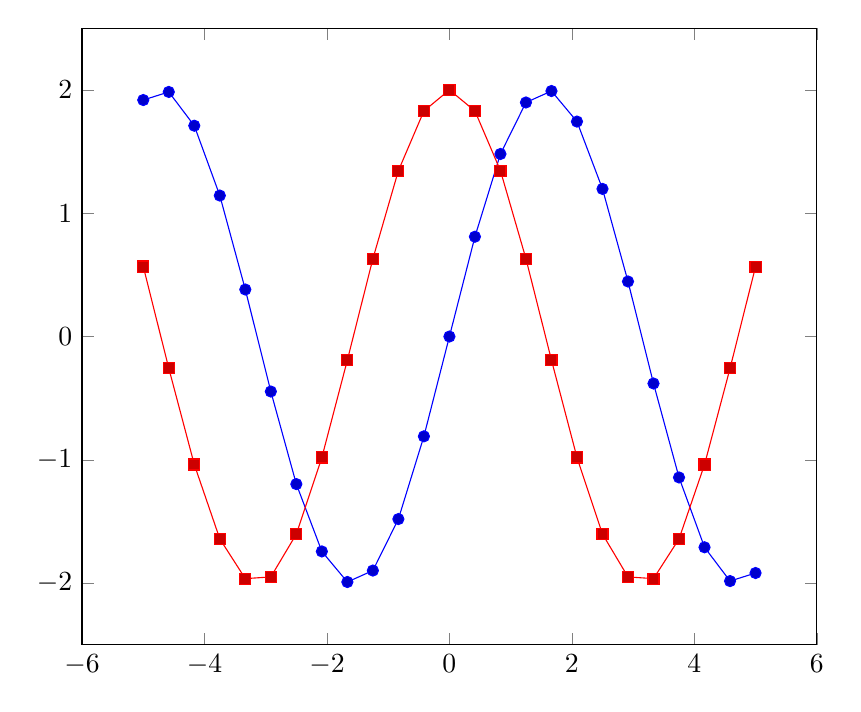
\begin{tikzpicture}
            \begin{axis}[ylabel={}, ymin=-2.5, ymax=2.5, width=.9\textwidth]
                \addplot{2*sin(deg(x))};
                \addplot{2*cos(deg(x))};
            \end{axis}
        \end{tikzpicture}
    \end{minipage}
    \begin{minipage}[b]{.45\textwidth}
        \begin{tikzpicture}
            \begin{axis}[ymin=-2.5, ymax=2.5, width=.9\textwidth]
                \addplot[green]{max(2*sin(deg(x)) - \vgamma, 2*cos(deg(x)) - \vgamma, 0)};
            \end{axis}
        \end{tikzpicture}
    \end{minipage}
\end{figure}

\noindent Se si volesse estendere questo circuito per trovare il massimo tra tre ingressi, si potrebbe tranquillamente
fare aggiungendo un' altro ramo in ingresso.

Nel caso in cui $V_1$ e $V_2$ siano segnali digitali, ovvero che possono solo assumere due valori $V_h$ e $V_l$, il circuito
si comporta come una porta logica \textbf{OR}.

\newpage
\subsection{Circuito rivelatore di minimo}
\begin{figure}[h]
    \centering
    \begin{circuitikz}
        \draw (0, 0) node[ground]{}
        to[battery1, label=$V_b$] (0, 1)
        to[R] (0, 3)
        to[diode, label=$D_2$] (-2, 3)
        node[circ, label={180:$V_2$}]{}

        (0, 3)
        -- (0, 4)
        to[diode, n=d1] (-2, 4)
        node[circ, label={180:$V_1$}]{}

        (d1.s) node[above]{$D_1$}
        (0, 3) node[circ, label={0:$V_u$}]{}
        ;
    \end{circuitikz}
\end{figure}

\begin{tcolorbox}[title=Relazioni fondamentali]
    \begin{align*}
        V_{d1} = V_u - V_1\\
        V_{d2} = V_u - V_2\\
        I = I_1 + I_2\\
        V_R = R \cdot I = V_b - V_u
    \end{align*}
\end{tcolorbox}

\begin{minipage}[b]{.45\textwidth}
    \begin{tcolorbox}[title=D1 e D2 OFF]
        \[\begin{cases}
            V_u = V_b\\
            V_1 > V_b - V_\gamma\\
            V_2 > V_b - V_\gamma\\
        \end{cases}\]
    \end{tcolorbox}
\end{minipage}
\begin{minipage}[b]{.45\textwidth}
    \begin{tcolorbox}[title=D1 ON e D2 OFF]
        \[\begin{cases}
            V_u = V_1 + V_\gamma\\
            V_1 < V_b - V_\gamma\\
            V_1 < V_2
        \end{cases}\]
    \end{tcolorbox}
\end{minipage}

\begin{minipage}[b]{.45\textwidth}
    \begin{tcolorbox}[title=D1 OFF e D2 ON]
        \[\begin{cases}
            V_u = V_2 + V_\gamma\\
            V_2 < V_b - V_\gamma\\
            V_2 < V_1
        \end{cases}\]
    \end{tcolorbox}
\end{minipage}
\begin{minipage}[b]{.45\textwidth}
    \begin{tcolorbox}[title=D1 e D2 ON]
        \[\begin{cases}
            V_u = V_1 + V_\gamma\\
            V_1 = V_2\\
            V_1 < V_b - V_\gamma
        \end{cases}\]
    \end{tcolorbox}
\end{minipage}

Quando entrambi i segnali di ingresso sono superiori a $V_b - V_\gamma$, entrambi i diodi sono spenti e la tensione coincide con $V_b$.
Se la tensione $V_1$ scende al di sotto di $V_b - V_\gamma$ ed è minore di $V_2$, allora l'uscita segue $V_1$ a meno di una
costante $V_\gamma$.
Stesso succede quando $V_2$ scende al di sotto di $V_b - V_\gamma$.
Se entrambe le tensioni di ingresso hanno lo stesso valore e sono al di sotto di $V_b - V_\gamma$, entrambi i diodi sono accesi
e l'uscita segue l'uno o l'altro a meno di una costante.

L'uscita $V_u$ può essere vista come $V_u = \min\big\{V_1 + V_\gamma, V_2 + V_\gamma, V_b\big\}$.

\begin{figure}[h]
    \centering
    \begin{minipage}[b]{.45\textwidth}
        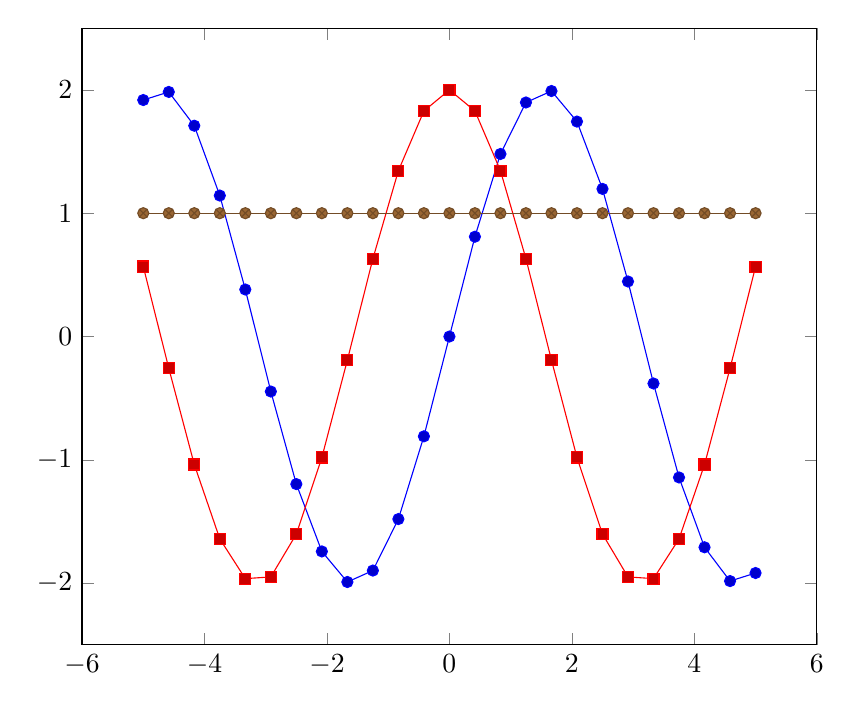
\begin{tikzpicture}
            \begin{axis}[ylabel={}, ymin=-2.5, ymax=2.5, width=.9\textwidth]
                \addplot{2*sin(deg(x))};
                \addplot{2*cos(deg(x))};
                \addplot{1};
            \end{axis}
        \end{tikzpicture}
    \end{minipage}
    \begin{minipage}[b]{.45\textwidth}
        \begin{tikzpicture}
            \begin{axis}[ymin=-2.5, ymax=2.5, width=.9\textwidth]
                \addplot[green, samples=50]{min(2*sin(deg(x)) + \vgamma, 2*cos(deg(x)) + \vgamma, 1)};
            \end{axis}
        \end{tikzpicture}
    \end{minipage}
\end{figure}

Se si fa riferimento a segnali di tipo digitale, il circuito si comporta come una porta logica \textbf{AND}.

\subsection{Circuito limitatore di tensione superiore ed inferiore}
Negli ultimi due esempi abbiamo dovuto analizzare quattro casi, uno per ogni zona possibile in cui
i due diodi del circuito potevano trovarsi. È evidente quindi, che nel caso più generale, con $n$ diodi
presenti nel circuito, il numero di casi da analizzare crescerebbe come $2^n$.
Quello che è importante da osservare è che non tutte le combinazioni sono significative dal punto di vista
fisico.
Alcune di esse possono essere escluse facendo ragionamenti a priori.

\begin{figure}[h]
    \centering
    \begin{circuitikz}[scale=1.5]
        \draw (0, 0) node[ground]{}
            -- (-1, 0)
            to[american voltage source, v=$V_i$] (-1, 2)
            to[R, i=$I$, v^=$V_R$] (1, 2)
            -- (2, 2)
            to[diode, label=$D_2$, i=$I_2$] (2, 0)
            -- (0, 0)

            (1, 0) to[diode, label=$D_1$, i=$I_1$] (1, 2)

            (1, 2) node[circ, label=$V_u$]{};

    \end{circuitikz}
\end{figure}

\begin{tcolorbox}[title=Equazioni generali]
    \begin{align*}
        &V_u + I \cdot R = V_i\\
        &V_1 = - V_u\\
        &V_2 = V_u\\
        &I + I_1 = I_2
    \end{align*}
\end{tcolorbox}

\begin{minipage}[b]{.45\textwidth}
    \begin{tcolorbox}[title=D1 e D2 OFF]
        \[\begin{cases}
            V_i = V_u\\
            V_i < V_\gamma\\
            V_i > -V_\gamma
        \end{cases}\]
    \end{tcolorbox}
\end{minipage}
\begin{minipage}[b]{.45\textwidth}
    \begin{tcolorbox}[title=D1 ON e D2 OFF]
        \[\begin{cases}
            V_u = -V_\gamma\\
            \\
            V_i < -V_\gamma
        \end{cases}\]
    \end{tcolorbox}
\end{minipage}

\begin{minipage}[b]{.45\textwidth}
    \begin{tcolorbox}[title=D1 OFF e D2 ON]
        \[\begin{cases}
            V_u = V\gamma\\
            \\
            V_i > V_\gamma
        \end{cases}\]
    \end{tcolorbox}
\end{minipage}
\begin{minipage}[t]{.45\textwidth}
    \begin{tcolorbox}[title=D1 e D2 ON]
        \color{red}
        \[\begin{cases}
            V_u = -V\gamma\\
            V_u = V\gamma\\
            \text{Non verificabile}
        \end{cases}\]
    \end{tcolorbox}
\end{minipage}

\begin{figure}[h]
    \centering
    \begin{minipage}[b]{.45\textwidth}
        \begin{tikzpicture}
            \begin{axis}[ymin=-2.5, ymax=2.5, width=.9\textwidth]
                \addplot[domain=-\vgamma:\vgamma]{x};
                \addplot[domain=-5:-\vgamma]{-\vgamma};
                \addplot[domain=\vgamma:5]{\vgamma};
            \end{axis}
        \end{tikzpicture}
    \end{minipage}
    \begin{minipage}[b]{.45\textwidth}
        \begin{tikzpicture}[
                declare function={
                    func(\x)= (\x < -\vgamma) * (-\vgamma) +
                                (\x > \vgamma) * \vgamma +
                                and(\x > -\vgamma, \x < \vgamma) * \x;
                }]
            \begin{axis}[ymin=-2.5, ymax=2.5, width=.9\textwidth]
                \addplot[samples=30] {func(sin(deg(x)))};
            \end{axis}
        \end{tikzpicture}
    \end{minipage}
\end{figure}
\noindent Al momento dell'impostazione delle equazioni generali, si poteva direttamente notare che $V_1 = -V_2$, quindi entrambi
i diodi non potevano essere accesi allo stesso tempo.
\\
Per modificare le due soglie del raddrizzatore basta mettere in serie nel circuito due generatori di tensione.

\newpage
\subsection{Raddrizzatore a doppia semionda}
\begin{figure}[h]
    \centering
    \begin{circuitikz}[scale=1.3]
        \draw (-1, 0)
        to[american voltage source, v=$V_i$] (-1, 3)
        -- (2, 3)
        to[diode, n=d1] (1, 1.5)
        node[circ, label={180:$V_u$}]{}
        to[R, i=$I_R$] (3, 1.5)
        to[diode, n=d4] (2, 0)
        to[diode, n=d3] (1, 1.5)

        (3, 1.5) to[diode, n=d2] (2, 3)
        (-1, 0) -- (2, 0)
        (3, 1.5) -- ++(0.5, 0) node[ground]{}

        %Labels
        (d1.s) node[left, label=$D_1$]{}
        (d2.s) node[right, label={$D_2$}]{}
        (d3.s) node[right, label={180:$D_3$}]{}
        (d4.s) node[right, label={-45:$D_4$}]{}
        ;
    \end{circuitikz}
\end{figure}

\noindent Dal numero di diodi presenti nel circuito mi attendo $2^4 = 16$ combinazioni delle regioni di funzionamento del circuito.
% Lezione 4 a 22 min

\begin{tcolorbox}[title=Equazioni Generali]
    \begin{align*}
    &I = I_1 - I_2 = I_3 - I_4\\
    &V_i = V_1 + V_R + V_4\\
    &-V_i = V_3 + V_R + V_2\\
    &I_R = I_2 + I_4\\
    &I_R = I_3 + I_1\\
    &V_u + V_1 + V_2 = 0\\
    &V_u + V_3 + V_4 = 0
    \end{align*}
\end{tcolorbox}

\noindent Risolvendo il circuito, otteniamo che le uniche soluzioni che hanno senso fisico sono le seguenti:
\\[10pt]
\begin{minipage}{.32\textwidth}
    \begin{tcolorbox}[title={D1,D4 OFF\\D2,D3 ON}]
        \[\begin{cases}
            V_u = -2 V_\gamma - V_i\\
            \\
            V_i < -2 V_\gamma\\
        \end{cases}\]
    \end{tcolorbox}
\end{minipage}
\begin{minipage}{.33\textwidth}
    \begin{tcolorbox}[title={D1,D2\\D3,D4 OFF}]
        \[\begin{cases}
            V_u = 0\\
            V_i < 2V_\gamma\\
            V_i > -2 V_\gamma
        \end{cases}\]
    \end{tcolorbox}
\end{minipage}
\begin{minipage}{.32\textwidth}
    \begin{tcolorbox}[title={D1,D4 ON\\D2,D3 OFF}]
        \[\begin{cases}
            V_u = Vi - 2 V_\gamma\\
            \\
            V_i > 2 V_\gamma
        \end{cases}\]
    \end{tcolorbox}
\end{minipage}

\noindent Il circuito ha un comportamento analogo al raddrizzatore a singola semionda, ha di diverso un tratto a pendenza negativa.
Ciò significa che per un valore negativo di $V_i < V_\gamma$, l'uscita assume il valore positivo opposto.
Quindi a differenza del circuito a singola semionda, che taglia la semionda negativa, questo circuito la trasforma in semionda positiva.
\begin{figure}[h]
    \centering
    \begin{minipage}[b]{.45\textwidth}
        \begin{tikzpicture}
            \begin{axis}[ymin=-2, ymax=4, width=.9\textwidth]
                \addplot[domain=(-2 * \vgamma):(2*\vgamma)]{0};
                \addplot[domain=(2 * \vgamma):5]{x-2*\vgamma};
                \addplot[domain=-5:-2*\vgamma]{-x-2*\vgamma};
                \addplot[dashed, clr-gray] coordinates {(2*\vgamma, 5) (2*\vgamma, -5)};
                \addplot[dashed, clr-gray] coordinates {(-2*\vgamma, 5) (-2*\vgamma, -5)};

                \node[circ,label={-45:{$2V_\gamma$}}] at (axis cs:2*\vgamma,0) {};
                \node[circ,label={180+45:{$-2V_\gamma$}}] at (axis cs:-2*\vgamma,0) {};
            \end{axis}
        \end{tikzpicture}
    \end{minipage}
    \begin{minipage}[b]{.45\textwidth}
        \begin{tikzpicture}[
            declare function={
                func(\x) = (\x < -2*\vgamma) * (-\x -2*\vgamma) +
                (\x > (2*\vgamma)) * (\x -2* \vgamma);
            }]
            \begin{axis}[ymin=-2, ymax=4, width=.9\textwidth]
                \addplot[samples=30] {func(3*sin(deg(x)))};
            \end{axis}
        \end{tikzpicture}
    \end{minipage}
\end{figure}

\noindent Il circuito raddrizzatore a doppia semionda è utilizzato per la trasformazione da corrente alternata a corrente continua.

\newpage
% Lezione 5
\subsection{Rivelatore di cresta}
Quando ho in ingresso un segnale sinusoidale (a valor medio nullo), tutti i circuiti raddrizzatori visti fino ad ora,
hanno la caratteristica di aver il valor medio della tensione in uscita, maggiore di zero.
In particolare nel caso del raddrizzatore a doppia semionda, la trasformazione delle semionde negative, contribuisce
ulteriormente al valor medio risultando in un valore maggiore rispetto al raddrizzatore a singola semionda.
È stato anche accennato che questi circuiti sono utilizzati per la trasformazione di corrente alternata in corrente continua,
resta comunque visibile dai grafici, che il segnale ottenuto in uscita dai circuiti è periodico e non
assimilabile ad un segnale di tensione continua.

Quello che vogliamo ottenere ora è estrarre il valor medio della tensione dal segnale periodico in uscita.
Attraverso le serie di Fourier possiamo ricostruire una qualunque funzione periodica attraverso una combinazione lineare di
toni sinusoidali a frequenza decrescente.

In particolare ricordiamo che tra le armoniche ottenute dalla serie di Fourier, l'armonica con frequenza di $0Hz$ rappresenta
il valor medio del segnale.
Il nostro obbiettivo diventa quindi quello di isolare la componente continua. Possiamo fare ciò attraverso un filtro
passa-basso capace di fare passare le componenti a frequenza più bassa, filtrando quelle a frequenza più alta.

\begin{figure}[h]
    \centering
    \begin{circuitikz}
        \draw
            (0, 0) node[ground]{}
            -- (-1, 0)
            to [sinusoidal voltage source, v=$V_i$, i=I] (-1, 2)
            to [diode, v^=$V_d$, i=$I_D$] (+2, 2)
            node[circ, label=$V_u$]{}
            to [R, i=$I_R$](2, 0)
            -- (0, 0)

            (2, 2)
            -- (3.5, 2)
            to[capacitor, i=$I_c$] (3.5, 0)
            -- (2, 0)
            ;
    \end{circuitikz}
    \caption{Raddrizzatore a singola semionda con filtro passa-basso}
\end{figure}


\begin{tcolorbox}[title=Equazioni Generali]
    \begin{align*}
        I_D = I_R + I_C\\
        I_R = \frac{V_u}{R}  \\
        I_C = C \frac{dV_u}{dt}
    \end{align*}
\end{tcolorbox}

\def\toff{t_{\text{off}}}
\def\wtoff{\omega \toff}

Nel caso del diodo acceso, il termine $\frac{V_u}{R}$, è positivo se $V_u$ è positivo, quindi fino a quando siamo nel $1^\circ$ o $2^\circ$ quadrante.
Mentre il secondo termine, essendo derivata di $V_u$ è negativa in caso di segnale decrescente. Quindi il diodo è sicuramente acceso
nell'intervallo $[0;\pi/2]$, mentre è sicuramente spento nell'intervallo $[\pi;\frac{3}{4}\pi]$.

Indichiamo con $\wtoff$ il punto appartenente a $]\pi/2;\pi[$ in cui il diodo passa dallo stato ON allo stato OFF.
Il punto $\wtoff$ è facilmente calcolabile osservando che corrisponde al punto di spegnimento, quindi dal passaggio di
$I_D > 0$ a $I_D = 0$.

\begin{tcolorbox}
    \begin{align*}
        &\begin{rcases}
            V_d = V_\gamma\\
            V_i - V_d - V_u = 0\\
            V_i = V_M \sin(\omega t)
        \end{rcases} \Rightarrow
        \begin{cases}
            V_u = V_M \sin(\omega t) - \cancelto{\text{trascurabile}}{V\gamma}\\
            \frac{dV_u}{dt} = V_M\cos(\omega t)\omega
        \end{cases}
        \\
        \\
        &I_D = \frac{V_M \sin(\omega t)}{R} + C V_M \omega \cos(\omega t)
        \\
        \\
        &\sin(\wtoff) + CR \omega \cos(\wtoff) = 0
        \\
    \end{align*}
\end{tcolorbox}

\noindent Siccome il punto che cerchiamo appartiene all'intervallo $]\pi/2;\pi[$, possiamo tranquillamente dire che
$\wtoff = \arctan(-CR\omega)$, tenendo presente di prendere la soluzione in tale intervallo. Osserviamo inoltre il
fatto che per $\omega RC$ crescente, il punto $\wtoff$ tende a $\pi/2$.
\\
Per il caso di diodo basta risolvere l'equazione differenziale $\frac{V_u}{R} + C\frac{dV_u}{dt} = 0$, ottenendo:
\\[10pt]
\begin{minipage}{.45\textwidth}
    \begin{tcolorbox}[title=Diodo ON]
        \[\begin{cases}
            \tan(\omega t) > - CR\omega\\
            V_u = V_M \sin(\omega t) - \cancelto{\text{trascurabile}}{V\gamma}
        \end{cases}\]
    \end{tcolorbox}
\end{minipage}
\begin{minipage}{.45\textwidth}
    \begin{tcolorbox}[title=Diodo OFF]
        \[\begin{cases}
            V_u(t) = V_u(\toff) e^{-\frac{1}{RC}(t - \toff)}\\
            V_u > V_M \sin (\omega t) - \cancelto{\text{trascurabile}}{V\gamma}
        \end{cases}\]
    \end{tcolorbox}
\end{minipage}

\noindent Quindi al momento di spegnimento del diodo, l'andamento della tensione decade seguendo l'andamento di
un esponenziale negativo.

\begin{figure}[h]
    \centering
    \def\tf{5*180/8}

    \begin{tikzpicture}[
        declare function={
            vi(\x) = 5*sin(\x);
            func(\x) = max(
                    (\x > \tf) * vi(\tf) * exp((\tf - \x)/250),
                    vi(\tf) * exp((\tf - \x - 360)/250),
                    vi(\x)
            ) - \vgamma;
        }]
        \begin{axis}[xmin=-1, xmax=10]
            \addplot [clr-main-red, samples=40, domain=-1:10] {vi(deg(x))};
            \addplot [clr-main-blue, samples=100, domain=-1:10] {func(mod(deg(x) + 360, 360))};
        \end{axis}
    \end{tikzpicture}
\end{figure}

\noindent L'effetto della capacità diventa quindi evidente,
La presenza della capacità fa si che il diodo si spenga prima, tanto prima quanto più elevata la capacità, ed una volta
che si è spento la tensione non segue più la sinusoide ma un esponenziale decrescente con costante di
tempo dipendente da RC. Maggiore è il prodotto RC, minore è il decadimento.

L'idea di partenza era quella di trasformare la tensione alternata in tensione continua, e per RC sufficientemente grande,
siamo in grado di approssimare un generatore di tensione continua.

Questo circuito può essere utilizzato anche come un demodulatore di ampiezza, portando l'uscita a seguire l'andamento
dell'ampiezza della sinusoide in ingresso.

\newpage
% Lezione 6
\subsection{Diodi in regime dinamico}
\label{sec:regime_dinamico}
Fin'ora abbiamo tracciato delle caratteristiche di trasferimento ingresso-uscita, presupponendo che in ogni istante
fosse possibile determinare la tensione d'uscita in funzione di quella in ingresso indipendentemente dal tempo, come
se fosse una relazione statica.
Ma nel diodo, per passare dalla condizione di polarizzazione diretta, alla condizione di polarizzazione inversa, è necessario
che avvenga uno spostamento di carica all'interno del dispositivo, ed è impossibile muovere della carica in tempi nulli.
\\
Quindi ad ogni variazione di carica, è associato un ritardo.

Vogliamo stimare questo ritardo per capire se i risultati sino ad ora calcolati sono effettivamente realistici o devono
essere a loro volta corretti alla luce di questa considerazione.

\begin{figure}[h]
    \centering
    \begin{minipage}{.45\textwidth}
        \begin{circuitikz}
            \draw
                (0, 0) node[ground]{}
                -- (-1, 0)
                to [american voltage source, v=$V_i$, i=I] (-1, 2)
                to [diode, i=$I_D$] (2, 2)
                to [R, v^=$V_u$](2, 0)
                -- (0, 0)
                ;
            \draw[clr-main-blue]
                (-0.5, 2) -- ++(0, 1.5)
                to[polar capacitor, color=clr-main-blue, i=$I_C$] ++(2, 0)
                -- ++(0, -1.5)
                ;
        \end{circuitikz}
    \end{minipage}
    \begin{minipage}{.45\textwidth}
        \begin{tikzpicture}
            \begin{axis}[ylabel=$V$, xlabel=$t$, ymin=-4, ymax=4, xmin=-4, xmax=4]
                \addplot [clr-main-blue] coordinates {(-5, 2) (0, 2)};
                \addplot [clr-main-blue] coordinates {(0, -2) (5, -2)};
                \addplot [clr-gray] coordinates {(-5, 2-\vgamma) (0, 2-\vgamma)};
                \addplot [clr-gray] coordinates {(0, 0) (5, 0)};

                \addplot [clr-main-red] coordinates {(3, -2) (3, 2)};
                \addplot [clr-main-red] coordinates {(3, 2) (5, 2)};

                \node [right, clr-gray] at (0, 2-\vgamma) {$V_u$};
                \node [right, clr-main-blue] at (0, 2) {$V_i$};
                \node [above] at (-2, 2) {ON};
                \node [above] at (2, 0) {OFF};
            \end{axis}
        \end{tikzpicture}
    \end{minipage}
\end{figure}

In grigio riportata la risposta statica del circuito al segnale $V_i$ in ingresso.

Per calcolare il ritardo di propagazione è necessario introdurre in parallelo al diodo ideale una capacità parassita,
permettendo di simulare il comportamento di un componente reale.

La relazione associata alla carica di questo condensatore parassita non è descritta dalla relazione $Q=CV$, ma da una
relazione lineare, dove nel primo quadrante segue la relazione esponenziale $Q = Q_s (e^{V_d / V_t} - 1)$.
Si può notare come il rapporto $Q/I_D = Q_s / I_s = \tau$ è costante, con le dimensioni fisiche di un tempo.

Sintetizziamo quindi la regione di funzionamento della capacità in funzione diretta, come $Q=\tau I$.

La stessa relazione non vale in polarizzazione inversa, dove la carica non segue un asintoto, ma ha un' andamento
simile a quello di una radice quadrata.

Dato che abbiamo approssimato l'andamento della corrente con un andamento lineare a tratti, faremo lo stesso con la carica.
È del tutto evidente che la qualità di questa approssimazione è meno accurata in regione di polarizzazione inversa,
buona ma ci accontenteremo, mettendo in evidenza quando questa approssimazione risulti troppo imprecisa.

\begin{minipage}{.45\textwidth}
    \begin{tcolorbox}[title=Diodo OFF]
        \[\begin{cases}
            I_D = 0\\
            Q = 0\\
            V_d < V_\gamma
        \end{cases}\]
    \end{tcolorbox}
\end{minipage}
\begin{minipage}{.45\textwidth}
    \begin{tcolorbox}[title=Diodo ON]
        \[\begin{cases}
            V_D = V_\gamma\\
            I_D > 0\\
            Q > 0
        \end{cases}\]
    \end{tcolorbox}
\end{minipage}

Ed è sempre valida la relazione $Q = \tau I$

Per $t < 0$ il circuito si trova in regione statica quindi è ancora descritto dalle relazioni statiche del diodo.
Stessa cosa accade per $t \to \infty$, dove la regione di transitorio tende ad esaurirsi.
\subsubsection{Analisi per $t < 0$}
Il circuito è descritto dalle relazioni statiche, e dalla tensione $V_i = V_f > V_\gamma$ si ricavano le relazioni:
\[\begin{cases}
    V_u = V_{f} - V_\gamma
    \\
    I = (V_{f} - V_\gamma)/R
    \\
    Q = \tau I = \frac{\tau}{R} (V_{f} - V_\gamma)
\end{cases}\]
\subsubsection{Analisi per $t \to \infty$}
Passato un tempo sufficientemente lungo, il circuito è ancora descritto dalle relazioni statiche,
e dalla tensione $V_i = -V_R < 0$:
\[\begin{cases}
    V_u = 0
    \\
    I = 0
    \\
    Q = 0
\end{cases}\]

\subsubsection{Analisi per $t > 0$}
\begin{tcolorbox}[title=Equazioni generali]
    \begin{align*}
        &V_i - V_d - V_u = 0\\
        &I_d + I_c = I\\
        &I_c = \frac{dQ_u}{dt}\\
        &Q = \tau I_D
    \end{align*}
\end{tcolorbox}
Analizzando il transitorio di scarica del condensatore parassita, la tensione in ingresso è $V_i = -V_R$, e la
carica, non potendo variare istantaneamente è ancora uguale al valore calcolato per $t < 0$. Quindi: $Q = \frac{\tau}{R}(V_f - V_\gamma)$.

Siccome $V_C = \frac{1}{C} Q$, se la carica non è variata, allora anche la tensione ai capi della capacità parassita è rimasta
costante.
Per $t < 0$, la tensione $V_C$ ai capi della capacità era pari a $V_\gamma$, (imposta dalla polarizzazione diretta dal diodo),
quindi segue che il valore iniziale della tensione di uscita è
$$V_u = V_i - V_\gamma = -V_R - V_\gamma$$

Che comporta un valore di corrente iniziale $I = -\frac{1}{R}(V_R + V_\gamma)$.

Nota la situazione iniziale, iniziamo l'analisi del transitorio. Dall'equazione $I_C + I_D = I$, otteniamo:
$$
    \frac{dQ}{dt} + \frac{Q}{\tau} = -\frac{V_R + V_\gamma}{R}
$$
Risolvendo l'equazione differenziale:
\begin{align}
    \frac{1}{dt} &= \big(-\frac{Q}{\tau} - \frac{V_R + V_\gamma}{R}\big)\frac{1}{dQ}
    \\
    \frac{1}{\tau} dt &= -\frac{R}{RQ + \tau (V_R + V_\gamma)} dQ
    \\
    -\frac{1}{\tau}\int_0^t{dt} &= \int_{Q(0)}^{Q(t)}{\frac{R}{Q + \tau (V_R + V_\gamma)} dQ}
    \\
    -\frac{1}{\tau} t &= \ln\Big(\frac{Q(t) + \frac{\tau}{R}(V_R + V_\gamma)}{Q(0) + \frac{\tau}{R}(V_R + V_\gamma)}\Big)
\end{align}

Sostituendo $Q(0) = \frac{\tau}{R}(V_f - V_\gamma)$ e risolvendo per $Q(t)$:
$$
    Q(t) = \frac{\tau}{R}(V_f + V_R) e^{-\frac{t}{\tau}} - \frac{\tau}{R}(V_R + V_\gamma)
$$
Si ottiene l'espressione di un'esponenziale decrescente, che tende asintoticamente ad un valore di carica negativo: $-\frac{\tau}{R}(V_R + V_\gamma)$.
L'equazione ottenuta è valida solo per $Q(t) > 0$.

Con questa osservazione, è possibile calcolare la durata totale del transitorio, imponendo $Q(t) = 0$.

\begin{align*}
    \frac{\tau}{R}(V_f + V_R) e ^ {-t_s/\tau} - \frac{\tau}{R}(V_R + V_\gamma) = 0
    \\
    t_s = \tau \ln\Big(\frac{V_f + V_R}{V_R + V_\gamma}\Big)
\end{align*}
Si vede subito che il rapporto è maggiore di 1, e che il tempo di storage, non dipende dal valore della resistenza,
ma dipende unicamente dalla escursione di tensione e dalle caratteristiche fisiche $\tau$ del diodo.

Questo significa che il diodo, dovendo smaltire la carica positiva sulla giunzione, per un certo periodo di tempo tiene costante
la tensione ai suoi capi, ritardando lo spegnimento.
Il tempo $t_s$ prende il nome di \textit{tempo di storage}.

\begin{center}
    \def\tm{3}

    \begin{minipage}{.32\textwidth}
        \begin{tikzpicture}
            \begin{axis}[width=.95\textwidth, ylabel=$V_u$, xlabel=$t$, xmin=-2, xmax=7]
                \addplot [clr-main-blue] coordinates {(-5, 3) (0, 3)};
                \addplot [clr-main-blue] coordinates {(0, -3) (\tm, -3)};
                \addplot [clr-main-blue] coordinates {(\tm, -3) (\tm, 0)};
                \addplot [clr-main-blue] coordinates {(\tm, 0) (8, 0)};
                \addplot [clr-main-red] coordinates {(\tm + 2, 0) (\tm + 2, 3)};
                \addplot [clr-main-red] coordinates {(\tm + 2, 3) (8, 3)};
            \end{axis}
        \end{tikzpicture}
    \end{minipage}
    \begin{minipage}{.31\textwidth}
        \begin{tikzpicture}
            \begin{axis}[width=.95\textwidth, ylabel=$I$, xlabel=$t$, xmin=-2, xmax=7]
                \addplot [clr-main-blue] coordinates {(-5, 3) (0, 3)};
                \addplot [clr-main-blue] coordinates {(0, -3) (\tm, -3)};
                \addplot [clr-main-blue] coordinates {(\tm, -3) (\tm, 0)};
                \addplot [clr-main-blue] coordinates {(\tm, 0) (8, 0)};
                \addplot [clr-main-red] coordinates {(\tm + 2, 0) (\tm + 2, 3)};
                \addplot [clr-main-red] coordinates {(\tm + 2, 3) (8, 3)};
            \end{axis}
        \end{tikzpicture}
    \end{minipage}
    \begin{minipage}{.32\textwidth}
        \begin{tikzpicture}
            \begin{axis}[width=.95\textwidth, ylabel=$Q$, xlabel=$t$, xmin=-2, xmax=8]
                \addplot [clr-main-blue] coordinates {(-5, 3) (0, 3)};
                \addplot [clr-main-blue, domain=0:\tm]{(3 / (1-e^(-\tm)))*e ^(-x) - (3 / (1-e^(-\tm))) +3};
                \addplot [clr-main-blue] coordinates {(\tm, 0) (8, 0)};
                \addplot [clr-main-red, domain=\tm+2:8] {-e^(-x + ln(3) + \tm+2) + 3};
            \end{axis}
        \end{tikzpicture}
    \end{minipage}
\end{center}

Nel modello approssimato che stiamo utilizzando si impiega un tempo $t_s$ per passare da $Q = Q(0^-)$, a $Q = 0$
perché abbiamo dovuto spostare le cariche interne al diodo fino ad arrivare al valore 0.
Siccome non sono necessari ulteriori spostamenti di carica, il transitorio rimanente è immediato, e la tensione varia istantaneamente.

Abbiamo già commentato che la qualità dell'approssimazione della carica è inferiore a quella della corrente, dato
che in regione di polarizzazione inversa, una si comporta come radice e l'altra come esponenziale negativo che tende ad un
valore di $I_s$ pressoché 0.

Questo significa che l'approssimazione che considera nulla la carica in polarizzazione inversa non è accurata, perché la
carica essendo anche debolmente negativa, comporta un transitorio di scarica del condensatore, dove ci dobbiamo aspettare che
il valore della resistenza $R$ influirà sul tempo di scarica.

Abbiamo descritto il transitorio di spegnimento del diodo, in due tratti:
il primo caratterizzato da una tensione costante $V_d = V_\gamma$ ed una carica che varia da un valore positivo
ad un valore nullo in un tempo $t_s$, ed un secondo tratto dove la carica è costante e vale 0,
e la tensione $V_d < V_\gamma$ che si compie in un tempo nullo.

Per determinare come funziona il passaggio di accensione del diodo, dovremo percorrere questi due tratti
all'inverso, entrambi descritti dalle stesse equazioni.
Dato che percorrendo il secondo tratto impieghiamo un tempo nullo, visto che non comporta spostamento di carica,
nel primo tratto avremo ai capi del diodo una tensione costante pari a $V_f - V_\gamma$.
Ma siccome non appena il condensatore comincia a caricarsi la tensione ai capi del diodo ha assunto già il suo
valore definitivo, il transitorio inverso ha un comportamento totalmente differente.
Mentre per spegnere il diodo è necessario un tempo di spegnimento $t_s$, per accendere il diodo (in termini di
tensione in uscita) il tempo di accensione non è visibile.

Il transitorio del diodo è asimmetrico, è lento a spegnersi e molto rapido ad accendersi.

Abbiamo stimato che il tempo di spegnimento del diodo è di circa $20ns$, e questo tempo è pressoché indipendente
dalla resistenza.

Le approssimazioni fatte sino ad ora sono del tutto accettabili quando il periodo del segnale è maggiore come
ordine di grandezza al ritardo intrinseco del diodo. Diventa non trascurabile quando le frequenze del segnale
sono notevolmente maggiori rispetto al ritardo. Al crescere della frequenza il capacitore tende a cortocircuitare
il diodo.

Esiste quindi un limite alla frequenza massima di commutazione che posso richiedere ad un diodo.
Questo è uno dei motivi per cui la frequenza di clock è limitata ad un valore massimo e che il periodo associato a
quella frequenza deve essere sufficientemente lungo per permettere ai transitori del
circuito di completarsi.

\end{document}
